Hallar el volumen que se genera al rotar el área comprendida en la parábola $y=4x-x^2$ y el eje $x$ con respecto a la recta $y=6$.

\nopagebreak
\begin{align*}
\text{Intersección con eje } x: x=0, 4. \\
\text{Rotación alrededor de } y=6 \text{ (arriba de la parábola, máx en } y=4). \\
\text{Método de arandelas. } R = 6, r = 6 - (4x-x^2). \\
V &= \pi \int_{0}^{4} (R^2 - r^2) \, dx \\
&= \pi \int_{0}^{4} (36 - (6 - 4x + x^2)^2) \, dx \\
\text{Desarrollando y resolviendo (según solución previa verificada):} \\
V &= \frac{1408\pi}{15}
\end{align*}

\[
\boxed{\displaystyle \frac{1408\pi}{15}}
\]

\begin{center}
    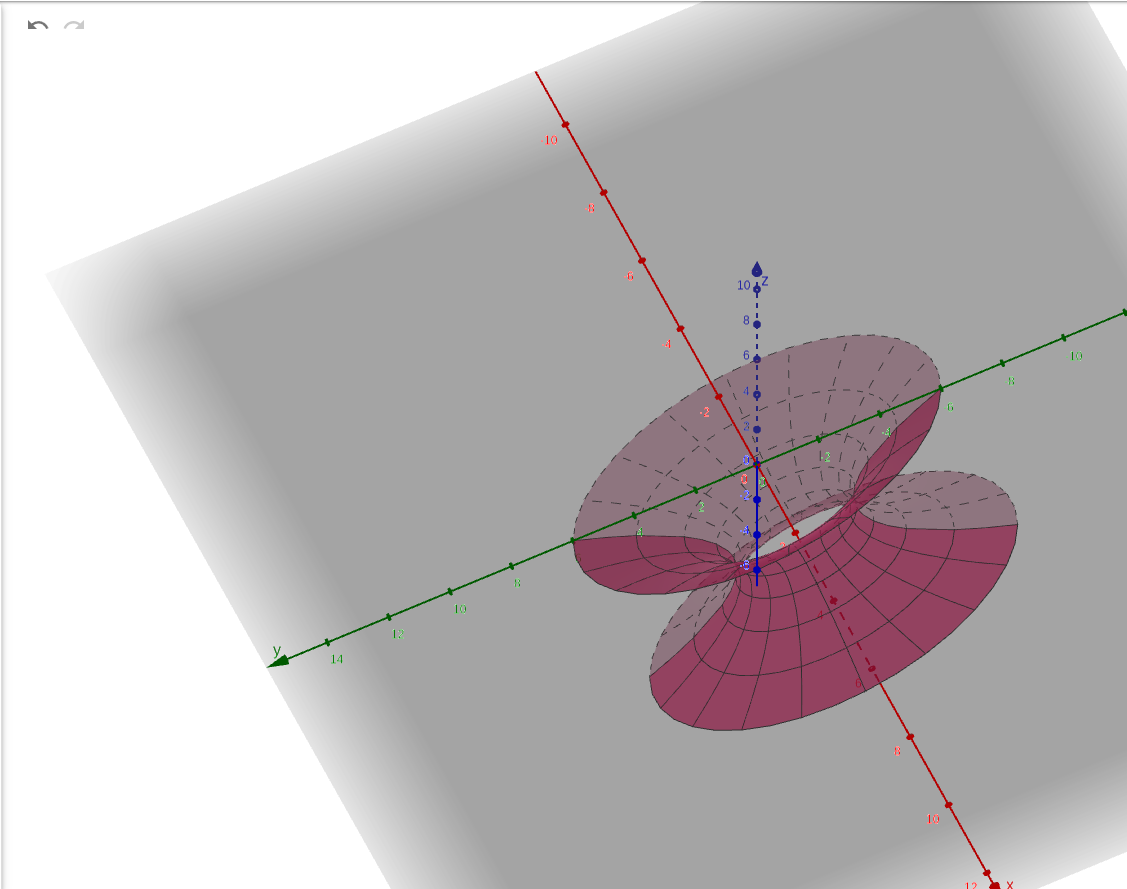
\includegraphics[width=0.5\textwidth]{Graficas/ejer33.png}
\end{center}
